\chapter{Data analysis}

\section{Simulation of survival data}

We wish to simulate survival times $\ti$ with censoring. We draw from some survival time distribution $f(\cdot)$. If the survival times have a closed form probability distribution function which is available in our chosen software package, we can draw from this distribution directly. To (right) censor the data, one typically draws a censoring time $W\sim f(\cdot)$, and let the observed survival times then be $\tilde{t}_i=\min(\ti,W)$, with corresponding $\di$ equal to 1 if the actual survival time was observed, i.e., if $\ti<W$. Crucially, this assumes independent censoring, i.e., that the censoring time is independent of the survival times. This does not pose a problem. Summary of the procedure:

\begin{algorithm}
\caption{Generate data}
\label{algo:sim}
\begin{enumerate}
    \item Make design matrices $\X$, $\Z$.
    \item Set $\bbeta$ and $\bgamma$.
    \item Link covariates and parameters using link functions
        \begin{align*}
            \ln y_0&=\bbeta^T\X \\
            \mu&=\bgamma^T\Z.
        \end{align*}
    \item Draw $N$ survival times $(t_i)_{i=1}^N$ from IG$(\mu,y_0)$.
    \item Draw a censoring time $W$ from some distribution.
    \item Right censor data by choosing $\widetilde{t}_i=\min(t_i,W)$. The indicator on whether observation $i$ was observed or not is then $\delta_i=I(\widetilde{t}_i=t_i)$.
    \item The simulated data set is $(t_i,\delta_i)$.
\end{enumerate}
\end{algorithm}

\begin{figure}[H]\centering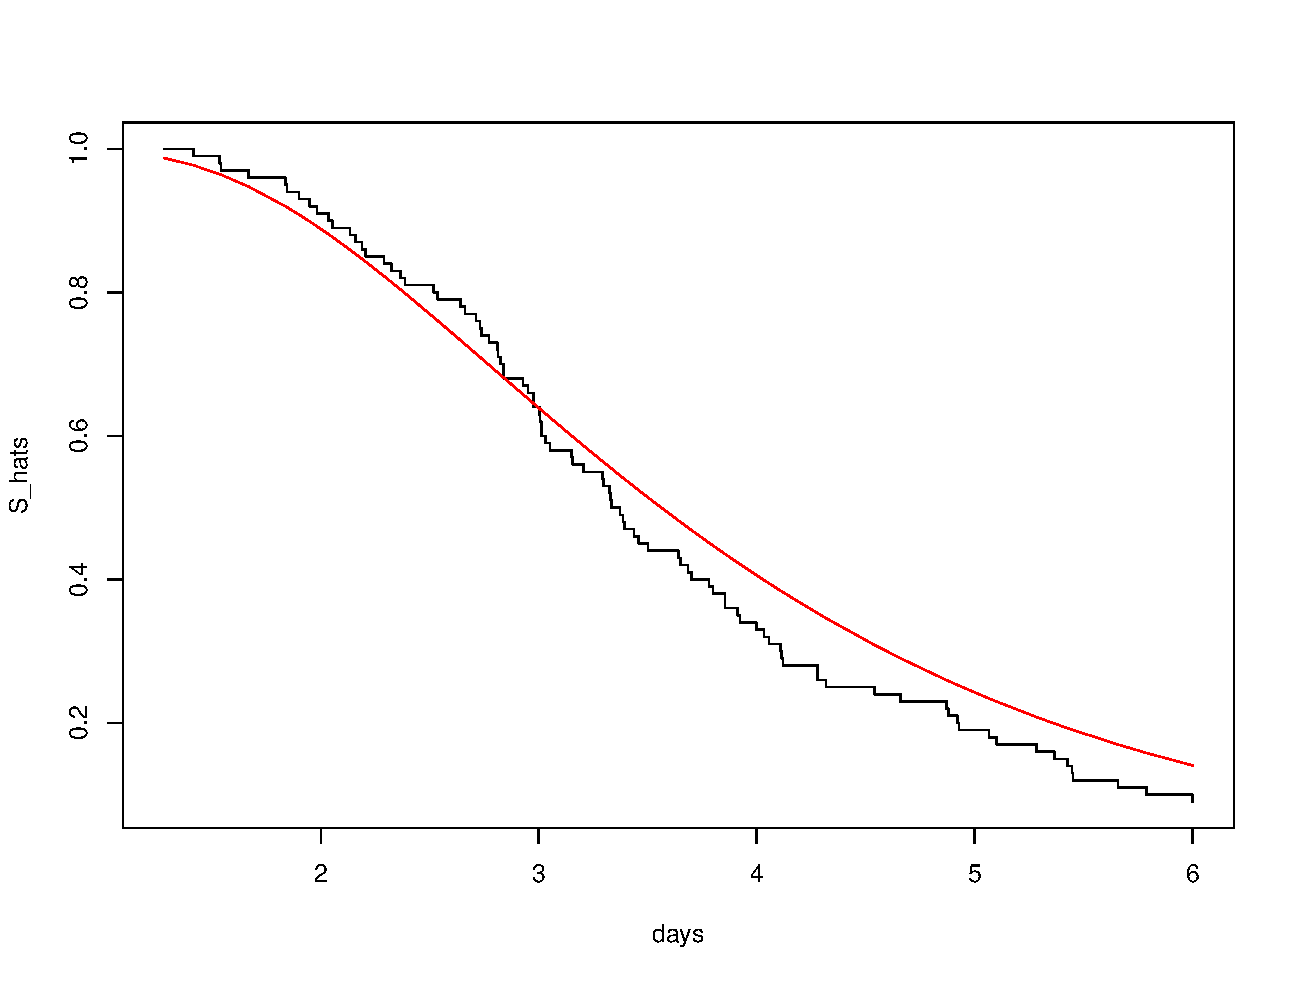
\includegraphics[height=9cm]
    {figures/simulated-IG.pdf}
\end{figure}
Experiment: Let $y_0=4$, $\mu=-1$. Draw 100 times from this. Censor at 6. Use numerical optimization routine to find maximizing parameters. Shown is the Kaplan-Meier empirical cumulative survival rate, and in red is the parametric survival curve with optimized $\hat{\mu}$ and $\hat{y_0}$. However, these are $\hat{y_0}=2.96$ and $\hat{\mu}=0.975$. I have also done similar experiments, where a negative $\mu$ is not picked up on.

\begin{figure}\centering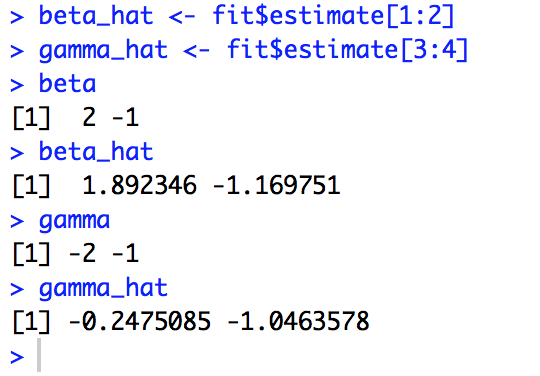
\includegraphics[height=6cm]
    {figures/params.png}
\end{figure}